\renewcommand{\theequation}{\theenumi}
\begin{enumerate}[label=\thesection.\arabic*.,ref=\thesection.\theenumi]
\numberwithin{equation}{enumi}
	%
%
%
%
%
\item Parallelograms on the same base (or equal bases) and between the same parallels are equal in area.
\item If a parallelogram and a triangle are on the same base and between the same parallels, then area of the triangle is half the area of the parallelogram.
%
\item  The quadrilateral formed by joining the mid-points of the sides of a quadrilateral, in order, is a parallelogram.
%
%
\item Two parallel lines l and m are intersected by a transversal p. Show that the quadrilateral formed by the bisectors of interior angles is a rectangle.
%
\item Show that the bisectors of angles of a parallelogram form a rectangle.
%
%
\item $ABCD$ is a parallelogram in which $P$ and $Q$ are mid-points of opposite sides $AB$ and $CD$. If $AQ$ intersects $DP$ at $S$ and $BQ$ intersects $CP$ at $R$, show that: 
%
\begin{enumerate}
\item  $APCQ$ is a parallelogram. 
\item $DPBQ$ is a parallelogram. 
\item $PSQR$ is a parallelogram.
\end{enumerate}
%
\item $l, m$ and $n$ are three parallel lines intersected by transversals $p$ and $q$ such that $l, m$ and $n$ cut off equal intercepts $AB$ and $BC$ on $p$ . Show that $l, m$ and $n$ cut off equal intercepts $DE$ and $EF$ on $q$ also.
%
\item Parallelograms on the same base (or equal bases) and between the same parallels are equal in area.
\item Area of a parallelogram is the product of its base and the corresponding altitude. 
\item Parallelograms on the same base (or equal bases) and having equal areas lie between the same parallels.
\item If a parallelogram and a triangle are on the same base and between the same parallels, then area of the triangle is half the area of the parallelogram.
\item In parallelogram $ABCD$, two points $P$ and $Q$ are taken on diagonal $BD$ such that $DP = BQ$. show that \begin{enumerate}
 \item  $\triangle  APD  \cong   \triangle  CQB$ 
\item $AP = CQ$ \item  $\triangle  AQB  \cong   \triangle  CPD$ 
\item $AQ = CP$ 
\item $APCQ$ is a parallelogram
\end{enumerate}
\item $ABCD$ is a parallelogram and $AP$ and $CQ$ are perpendiculars from vertices $A$ and $C$ on diagonal $BD$ . Show that 
\begin{enumerate} 
\item  $\triangle  APB  \cong   \triangle  CQD $ 
\item $AP = CQ$
\end{enumerate}
%
\item In  $\triangle  ABC$ and  $\triangle  DEF, AB = DE, AB  \parallel  DE, BC = EF$ and $BC  \parallel  EF$. Vertices $A, B$ and $C$ are joined to vertices $D, E$ and $F$ respectively. Show that 
\begin{enumerate}
\item quadrilateral $ABED$ is a parallelogram 
\item quadrilateral $BEFC$ is a parallelogram 
\item $AD  \parallel  CF$ and $AD = CF$ 
\item quadrilateral $ACFD$ is a parallelogram 
\item $AC$ = $DF$ 
\item  $\triangle  ABC  \cong   \triangle  DEF$.
%
\end{enumerate}

\item $ABCD$ is a trapezium in which $AB$  $\parallel$  $CD$ and $AD = BC$. Show that 
\begin{enumerate} 
\item$\angle A$ =  $\angle B$  
\item  $\angle C  =  \angle D$  \item  $\triangle  ABC  \cong   \triangle  BAD$ 
\item diagonal $AC$ = diagonal $BD$ 
\end{enumerate}
%
\item $ABCD$ is a quadrilateral in which $P, Q, R$ and $S$ are mid-points of the sides $AB, BC, CD$ and $DA$ $AC$ is a diagonal. Show that 
\begin{enumerate} 
\item $SR$  $\parallel$  $AC$ and $SR =\frac{1}{ 2}AC$
\item $PQ = SR$ 
\item  $PQRS$  is a parallelogram.
\end{enumerate}
%
\item $ABCD$ is a rhombus and  $P, Q, R$ and $S$  are the mid-points of the sides  $AB, BC, CD$ and $DA$ respectively. Show that the quadrilateral  $PQRS$  is a rectangle.
\item $ABCD$ is a rectangle and  $P, Q, R$ and $S$  are mid-points of the sides  $AB, BC, CD$ and $DA$ respectively. Show that the quadrilateral  $PQRS$  is a rhombus.
\item $ABCD$ is a trapezium in which $AB  \parallel  DC, BD$ is a diagonal and $E$ is the mid-point of $AD$. A line is drawn through $E$ $\parallel$  $AB$ intersecting $BC$ at $F$. Show that $F$ is the mid-point of $BC$.
\item In a parallelogram $ABCD$, $E$ and $F$ are the mid-points of sides $AB$ and $CD$ respectively . Show that the line segments $AF$ and $EC$ trisect the diagonal $BD$.
\item Show that the line segments joining the mid-points of the opposite sides of a quadrilateral bisect each other.
\item $ABCD$ is a parallelogram in which $P$ and $Q$ are mid-points of opposite sides $AB$ and $CD$. If $AQ$ intersects $DP$ at $S$ and $BQ$ intersects $CP$ at $R$, show that: 
%
\begin{enumerate}
\item  $APCQ$ is a parallelogram. 
\item $DPBQ$ is a parallelogram. 
\item $PSQR$ is a parallelogram.
\end{enumerate}
%
\item $l, m$ and $n$ are three parallel lines intersected by transversals $p$ and $q$ such that $l, m$ and $n$ cut off equal intercepts $AB$ and $BC$ on $p$ . Show that $l, m$ and $n$ cut off equal intercepts $DE$ and $EF$ on $q$ also.
%
\item Diagonal $AC$ of a parallelogram $ABCD$ bisects $\angle A$ . show that 
\begin{enumerate}
\item it bisects  $\angle C$  also, 
\item $ABCD$ is a rhombus.
\end{enumerate}
%
\item $ABCD$ is a rhombus. Show that diagonal $AC$ bisects $\angle A$ as well as  $\angle C$  and diagonal $BD$ bisects  $\angle B$  as well as  $\angle D$ .
\item $ABCD$ is a rectangle in which diagonal $AC$ bisects $\angle A$ as well as  $\angle C$ . Show that 
\begin{enumerate}
\item $ABCD$ is a square 
\item diagonal $BD$ bisects  $\angle B$  as well as  $\angle D$ .
%
\end{enumerate}

\item If $E,F,G$ and $H$ are respectively the mid-points of the sides of a parallelogram $ABCD$, show that
\begin{align}
ar \brak{EFGH} =
\frac{1}{ 2}
ar \brak{ABCD} .
\end{align}
%
\item $P$ and $Q$ are any two points lying on the sides $DC$ and $AD$ respectively of a parallelogram $ABCD$. Show that $ar (APB) = ar (BQC)$.
%
\item P is a point in the interior of a parallelogram $ABCD$. Show that
\begin{enumerate}
\item $ar (APB) + ar (PCD) = \frac{1}{ 2}ar (ABCD)$
\item $ar (APD) + ar (PBC) = ar (APB) + ar (PCD)$
\end{enumerate}
%
\item $PQRS$ and $ABRS$ are parallelograms and $X$ is any point on side $BR$. show that 
\begin{enumerate} 
\item $ar (PQRS) = ar (ABRS)$
\item $ar (AX S) = \frac{1}{ 2} ar (PQRS)$
\end{enumerate}
%
\item A farmer was having a field in the form of a parallelogram $PQRS$. She took any point $A$ on $RS$ and joined it to points $P$ and $Q$. In how many parts the fields is divided? What are the shapes of these parts? The farmer wants to sow wheat and pulses in equal portions of the field separately. How should she do it?
%
\item $ABCD$ is a quadrilateral and $BE  \parallel  AC$ and also $BE$ meets $DC$ produced at $E$. Show that area of $ \triangle  ADE$ is equal to the area of the quadrilateral $ABCD$.
%
\item $E$ is any point on median $AD$ of a  $\triangle  ABC$. Show that $ar (ABE) = ar (ACE)$.
\item  In a $\triangle ABC, E$ is the mid-point of median $AD$. Show that $ar (BED) = \frac{1}{ 4}ar(ABC)$ .
\item  Show that the diagonals of a parallelogram divide it into four triangles of equal area.
\item   $ABC$ and $ABD$ are two triangles on the same base $AB$. If line- segment $CD$ is bisected by $AB$ at $O$, show that $ar(ABC) = ar (ABD)$.
%
\item $D$, $E$ and $F$ are respectively the mid-points of the sides $BC, CA$ and $AB$ of a $ \triangle  ABC$. show that 
\begin{enumerate}
\item $BDEF$ is a parallelogram. 
\item $ar (BDEF) =
\frac{1}{ 2}
ar (ABC)$
\end{enumerate}
%
\item   Diagonals $AC$ and $BD$ of quadrilateral $ABCD$ intersect at $O$ such that $OB = OD$. If $AB = CD$, then show that 
\begin{enumerate}
\item $ar (DOC) = ar (AOB)$
 \item $ar (DCB) = ar (ACB)$
\item $ar (DEF) =
\frac{1}{ 4}
ar (ABC)$ 
\end{enumerate}
\item $D$ and $E$ are points on sides $AB$ and $AC$ respectively of $ \triangle  ABC$ such that $ar (DBC) = ar (EBC)$. Prove that $DE  \parallel  BC$.
\item $XY$ is a line parallel to side $BC$ of a $\triangle ABC$. If $BE  \parallel  AC$ and $CF  \parallel  AB$ meet $XY$ at $E$ and $F$ respectively, show that
$ar (ABE) = ar (ACF)$.
\item The side $AB$ of a parallelogram $ABCD$ is produced to any point $P$. A line through $A$ and parallel to $CP$ meets $CB$ produced at $Q$ and then parallelogram $PBQR$ is completed. Show that $ar ($ABCD$) = ar (PBQR)$. \item Diagonals $AC$ and $BD$ of a trapezium $ABCD$ with $AB  \parallel  DC$ intersect each other at $O$. Prove that $ar (AOD) = ar (BOC)$.
\item  $ABCDE$ is a pentagon. A line through $B$ parallel to $AC$ meets $DC$ produced at $F$. Show that 
\begin{enumerate}
\item $ar (ACB) = ar (ACF)$
 \item $ar (AEDF) = ar (ABCDE)$
. 
\end{enumerate}
\item A villager Itwaari has a plot of land of the shape of a quadrilateral. The Gram Panchayat of the village decided to take over some portion of his plot from one of the corners to construct a Health Centre. Itwaari agrees to the above proposal with the condition that he should be given equal amount of land in lieu of his land adjoining his plot so as to form a triangular plot. Explain how this proposal will be implemented.
\item $ABCD$ is a trapezium with $AB  \parallel  DC$. A line parallel to $AC$ intersects $AB$ at $X$ and $BC$ at $Y$. Prove that $ar (ADX) = ar (ACY)$.
\item  $AP  \parallel  BQ  \parallel  CR$. Prove that $ar (AQC) = ar (PBR)$.
\item Diagonals $AC$ and $BD$ of a quadrilateral $ABCD$ intersect at $O$ in such a way that $ar (AOD) = ar (BOC)$. Prove that $ABCD$ is a trapezium.
\item  $AB \parallel DC \parallel RP$.  $ar (DRC) = ar (DPC)$ and $ar (BDP) = ar (ARC)$. Show that both the quadrilaterals $ABCD$ and $DCPR$ are trapeziums.

\item Parallelogram $ABCD$ and rectangle $ABEF$ are on the same base $AB$ and have equal areas. Show that the perimeter of the parallelogram is greater than that of the rectangle.
\item  In $\triangle ABC$,  $D$ and $E$ are two points on $BC$ such that $BD = DE = EC$. Show that $ar (ABD) = ar (ADE) = ar (AEC)$.
\item $ABCD, DCFE$ and $ABFE$ are parallelograms. Show that ar$ (ADE) = ar (BCF)$.
\item  $ABCD$ is a parallelogram and $BC$ is produced to a point $Q$ such that $AD = CQ$. If $AQ$ intersect $DC$ at $P$, show that $ar (BPC) = ar (DPQ)$.
$ABC$ and $BDE$ are two equilateral triangles such that $D$ is the mid-point of $BC$. If $AE$ intersects $BC$ at$ F$, show that 
\begin{enumerate}
\item $ar (BDE) = \frac{1}{ 4} ar (ABC)$
\item $ar (BDE) = \frac{1}{ 2} ar (BAE)$
\item $ar (ABC) = 2 ar (BEC)$
 \item $ar (BFE) = ar (AFD)$ 
\item $ar (BFE) = 2 ar (FED)$
\item $ar (FED) =
\frac{1}{ 8}
ar (AFC)$
\end{enumerate}
\item Diagonals $AC$ and $BD$ of a quadrilateral $ABCD$ intersect each other at $P$. Show that $ar (APB)  \times  ar (CPD) = ar (APD)  \times  ar (BPC)$.
\item  $P$ and $Q$ are respectively the mid-points of sides AB and BC of a $\triangle ABC$ and $R$ is the mid-point of $AP$, show that 
\begin{enumerate}
\item $ar (PRQ) = \frac{1 }{2}ar (ARC) $
\item $ar (PBQ) = ar (ARC)$
\item $ar (RQC) =
\frac{3}{ 8}
ar (ABC)$
\end{enumerate}
%
\item $ABC$ is a right triangle right angled at $A$. $BCED$, $ACFG$ and $ABMN$ are
squares on the sides $BC, CA$ and $AB$ respectively. Line segment $AX \perp  DE$ meets $BC$ at $Y$. Show that 
\begin{enumerate}
\item $ \triangle  MBC \cong  \triangle  ABD$
\item $ar (BYXD) = ar (ABMN)$ \item $ar (CYXE) = 2 ar (FCB)$
\item $ar (BYXD) = 2 ar (MBC)$ 
\item $ \triangle  FCB \cong  \triangle  ACE$
\item $ar (CYXE) = ar (ACFG)$
\item  $ar (BCED) = ar (ABMN) + ar (ACFG)$
\end{enumerate}
\item $L$ is a point on the diagonal $AC$ of quadrilateral $ABCD$.  If LM || CB and LN || CD, prove that $\frac{AM}{AB}=\frac{ AN}{  AD}$
\item The angles of quadrilateral are in the ratio 3 : 5 : 9 : 13. Find all the angles of the quadrilateral.
%\\
%\solution
%The given curve 
\begin{align}
	y =\frac{1}{x-1}
\end{align}
can be expressed as 
\begin{align}
	xy - y - 1 = 0 \label{eq:solutions/1/14/eq:hyperbola}
\end{align}
Hence, we have
\begin{align}
	\vec{V} = \frac{1}{2}\myvec{0 & 1 \\ 1 & 0}, 
	\vec{u} = \frac{1}{2}\myvec{0 \\-1},
	f = -1
\end{align}
Since $\mydet{\vec{V}} < 0$, the equation \eqref{eq:solutions/1/14/eq:hyperbola} represents hyperbola.
To find the values of $\lambda_1$ and $\lambda_2$, consider the characteristic equation,
\begin{align}
	\mydet{\lambda\vec{I} - \vec{V}} &= 0\\
	\implies \mydet{\myvec{\lambda & 0\\0 & \lambda} - \myvec{0 & \frac{1}{2} \\ \frac{1}{2} & 0}} &= 0\\
	\implies \mydet{ \lambda & \frac{-1}{2} \\ \frac{-1}{2} & \lambda} &= 0\\
	\implies \lambda_1 &= \frac{1}{2} , \lambda_2 = \frac{-1}{2}
\end{align}
In addition, given the slope -1, the direction and normal vectors are given by 
\begin{align}
	\vec{m} = \myvec{1 \\ -1} \\
	\vec{n} = \myvec{ 1 \\ 1}
\end{align}
The parameters of hyperbola are as follows:
\begin{align}
	\vec{c} &= -\vec{V}^{-1}\vec{u} \\
	&= -\myvec{0 & 2\\ 2 & 0}\myvec{0 \\ -\frac{1}{2}} \\
	&= \myvec{1 \\ 0}\\
	axes &= \begin{cases}
	\sqrt{\frac{\vec{u}^T\vec{V}^{-1}\vec{u} - f}{\lambda_1}} = \sqrt{2}\\
 \sqrt{\frac{f-\vec{u}^T\vec{V}^{-1}\vec{u}}{\lambda_2}} = \sqrt{2}
\end{cases}
\end{align}
which represents the standard hyperbola equation,
\begin{align}
	\frac{x^2}{2} - \frac{x^2}{2} = 1
\end{align}
The points of contact are given by 
\begin{align}
  \tiny{K} &=\pm \sqrt{\frac{\vec{u}^T\vec{V}^{-1}\vec{u} - f}{\vec{n}^T\vec{V}^{-1}\vec{n}}}
  = \pm \frac{1}{2}\\
  \vec{q} &= \vec{V}^{-1}(k\vec{n}-\vec{u})\\
  \vec{q_1} &= \myvec{0 & 2\\2 & 0} \sbrak{\frac{1}{2}\myvec{1 \\ 1} - \myvec{0\\ \frac{-1}{2}}}\\
  &= \myvec{2 \\ 1}\\
  \vec{q_2} &= \myvec{0 & 2\\2 & 0} \sbrak{\frac{-1}{2}\myvec{1 \\ 1} - \myvec{0\\ \frac{-1}{2}}}\\
  &= \myvec{0 \\ -1}
\end{align} 
$\therefore$ The tangents are given by
\begin{align}
	\myvec{1 & 1} \brak{\vec{x} - \myvec{2 \\ 1}} = 0 \\
	\myvec{1 & 1} \brak{\vec{x} - \myvec{0 \\ -1}} = 0
\end{align}
The desired equations of all lines having slope -1 that are tangents to the curve $\frac{1}{x-1}, x \neq 1$ are given by
\begin{align}
	\myvec{1 & 1}\vec{x} &= 3 \\
	\myvec{1 & 1}\vec{x} &= -1 
\end{align}
The above results are verified in the following figure.
\begin{figure}[h!] \label{eq:solutions/1/14/fig:tangents}
	\centering
	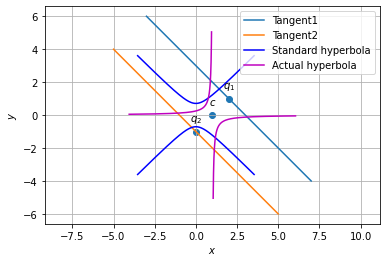
\includegraphics[width=\columnwidth]{./solutions/1/14/graph7.png}
	\caption{The standard and actual hyperbola.}
\end{figure}


\end{enumerate}
